\documentclass[10pt,a4paper]{article}
\usepackage[utf8]{inputenc}
\usepackage[portuguese]{babel}
\usepackage[T1]{fontenc}
\usepackage{amsmath}
\usepackage{amsfonts}
\usepackage{amssymb}
\usepackage{makeidx}
\usepackage{graphicx}
\usepackage{kpfonts}
\usepackage[left=3cm,right=2cm,top=3cm,bottom=3cm]{geometry}
\usepackage{float}
\usepackage{booktabs}
\usepackage{multirow}
\usepackage{dsfont}
\usepackage{empheq}
\newcommand{\MatR}[2]{{\mathcal{M}}_{#1\times #2}(\mathds{R})}
\DeclareMathOperator*{\argmin}{argmin}
\begin{document}
\section{Formulation and Discretization of the Problem of Pure Diffusion}

\begin{itemize}
\item Formulation:
\begin{alignat*}{3}
-(\kappa\phi')' & = s && \quad \text{ in } \Omega=]x_\frac{1}{2},x_{I+\frac{1}{2}}[\\
\phi & =\phi_{\text{lf},0} && \quad \text{ at } x=x_\frac{1}{2}\\
-\kappa\phi' & =\phi_{\text{rg},1} && \quad \text{ at } x=x_{I+\frac{1}{2}}
\end{alignat*}

\item Mesh:

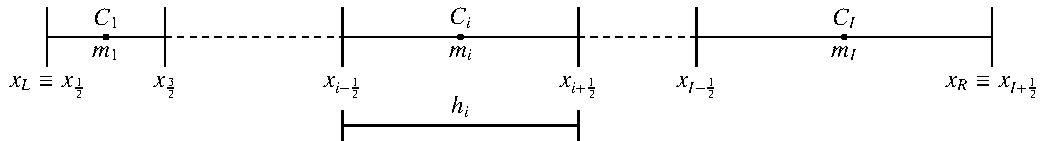
\includegraphics[width=\textwidth]{images/mesh_notation}

\item Discretization:
\begin{align*}
&-(\kappa\phi')'= s\\
&\int_{C_i}(-(\kappa\phi')')\,\text dx=\int_{C_i}s\,\text dx\\
&-(\kappa\phi')\big|_{x_{i-\frac{1}{2}}}^{x_{i+\frac{1}{2}}}=\int_{C_i}s\,\text dx\\
&-\left(\mathbb{F}_{\text D,i+\frac{1}{2}}-\mathbb{F}_{\text D,i-\frac{1}{2}}\right)=\mathbb{S}_i, \quad i=1,\ldots,I
\end{align*}
\end{itemize}

\section{Reconstructions and Matrices}
\begin{itemize}
\item At $x_\frac{1}{2}$:
\[
\phi_{\text d,\frac{1}{2}}(x)=\sum_{\alpha=0}^\text d \mathcal{R}_{\frac{1}{2},\alpha}(x-x_\frac{1}{2})^\alpha
\]

$\widehat{\mathcal{R}}_{\frac{1}{2}}=\left(\widehat{\mathcal{R}}_{\frac{1}{2},0},\ldots,\widehat{\mathcal{R}}_{\frac{1}{2},\text d}\right)^\text T$ is the solution of the constrained linear least squares problem

\begin{minipage}[c]{0.55\textwidth}
\begin{empheq}[box=\fbox]{align*}
\min & \quad
\sum_{j\in S_\frac{1}{2}} \omega_j\left [\frac{1}{h_j} \int_{C_j} \phi_{\text d,\frac{1}{2}}(x)\,\text dx -\phi_j \right]^2\\
\text{s.t.} & \quad \phi_{\text d,\frac{1}{2}}(x_\frac{1}{2})=\phi_{\text{lf},0}
\end{empheq}
\end{minipage}
\begin{minipage}[c]{0.025\textwidth}
$\Leftrightarrow$
\end{minipage}
\begin{minipage}[c]{0.35\textwidth}
\begin{empheq}[box=\fbox]{align*}
\min & \quad
\|A_\frac{1}{2} \mathcal R_\frac{1}{2} - B_\frac{1}{2}\|_2^2\\
\text{s.t.} & \quad C_\frac{1}{2} \mathcal R_\frac{1}{2}=D_\frac{1}{2}
\end{empheq}
\end{minipage}

So,
\begin{align*}
&\omega_j\left[\frac{1}{h_j}\int_{C_j}\phi_{\text d,\frac{1}{2}}\,\text dx-\phi_j\right]=0\\
\Leftrightarrow &\omega_j\left[\frac{1}{h_j}\int_{C_j}\phi_{\text d,\frac{1}{2}}\,\text dx\right]=\omega_j\phi_j\\\Leftrightarrow &\omega_j\left[\frac{1}{h_j}\int_{C_j}
\left(\sum_{\alpha=0}^\text d\mathcal{R}_{\frac{1}{2},\alpha}(x-x_{\text{lf}})^\alpha\right)\,\text dx\right]=\omega_j\phi_j\\
\Leftrightarrow &\omega_j\left[\frac{1}{h_j}\int_{C_j}
\left(\mathcal{R}_{\frac{1}{2},0}(x-x_{\text{lf}})^0+\mathcal{R}_{\frac{1}{2},1}(x-x_{\text{lf}})^1+\cdots+\mathcal{R}_{\frac{1}{2},\text d}(x-x_{\text{lf}})^\text d\right)\,\text dx\right]=\omega_j\phi_j\\
\Leftrightarrow &\omega_j\left[
\mathcal{R}_{\frac{1}{2},0}\underbrace{\left(\frac{1}{h_j}\int_{C_j}(x-x_{\text{lf}})^0\,\text dx\right)}_{A}+\mathcal{R}_{\frac{1}{2},1}\left(\frac{1}{h_j}\int_{C_j}(x-x_{\text{lf}})^1\,\text dx\right)+\cdots+\mathcal{R}_{\frac{1}{2},\text d}\left(\frac{1}{h_j}\int_{C_j}(x-x_{\text{lf}})^\text d\,\text dx\right)
\right]=\underbrace{\omega_j\phi_j}_B
\end{align*}
and,
\begin{align*}
& \phi_{\text d,\frac{1}{2}}(x_{\text{lf}})=\phi_{\text{lf},0}\\
\Leftrightarrow&\sum_{\alpha=0}^{\text d}\mathcal{R}_{\frac{1}{2},\alpha}(x_{\text{lf}}-x_{\text{lf}})^\alpha
=\phi_{\text{lf},0}\\
\Leftrightarrow&\mathcal{R}_{\frac{1}{2},0}\underbrace{(x_{\text{lf}}-x_{\text{lf}})^0}_C+\mathcal{R}_{\frac{1}{2},1}(x_{\text{lf}}-x_{\text{lf}})^1+\cdots+\mathcal{R}_{\frac{1}{2},\text d}(x_{\text{lf}}-x_{\text{lf}})^\text d=\underbrace{\phi_{\text{lf},0}}_{D}\\
\end{align*}



Then, the matrices are:
\begin{align*}
& A_\frac{1}{2}=[A_{\frac{1}{2},j\alpha}]\in \MatR{n_S}{(\text d+1)}=\omega_j\frac{1}{h_j}\int_{C_j}(x-x_{\frac{1}{2}})^\alpha\,\text dx\\
& B_\frac{1}{2}=[B_{\frac{1}{2},j}]\in \MatR{n_S}{1}=\omega_j\phi_j\\
& C_\frac{1}{2}=[C_{\frac{1}{2},j\alpha}]\in \MatR{1}{(\text d+1)}=
\begin{cases}
1 & \text{if}\quad \alpha=0\\
0 & \text{if}\quad \alpha=1,\ldots,\text d
\end{cases}\\
& D_\frac{1}{2}=[D_{\frac{1}{2},j}]\in \MatR{1}{1}=\phi_{\text{lf},0}
\end{align*}
%
\item At $x_\frac{3}{2},\ldots,x_{I-\frac{1}{2}}$:
\[
\phi_{\text d,i+\frac{1}{2}}(x)=\sum_{\alpha=0}^\text d \mathcal{R}_{i+\frac{1}{2},\alpha}(x-x_{i+\frac{1}{2}})^\alpha, 
\]


$\widetilde{\mathcal{R}}_{i+\frac{1}{2}}=\left(\widetilde{\mathcal{R}}_{i+\frac{1}{2},0},\ldots,\widetilde{\mathcal{R}}_{i+\frac{1}{2},\text d}\right)^\text T$ is the solution of the constrained linear least squares problem

\begin{minipage}[c]{0.55\textwidth}
\begin{empheq}[box=\fbox]{align*}
\min & \quad
\sum_{j\in S_{i+\frac{1}{2}}} \omega_j\left [\frac{1}{h_j} \int_{C_j} \phi_{\text d,i+\frac{1}{2}}(x)\,\text dx -\phi_j \right]^2
\end{empheq}
\end{minipage}


%\[
%\widetilde \phi_{\text d,i+\frac{1}{2}}=
%\min_{\widetilde{\mathcal{R}}_{i+\frac{1}{2},0},\>\ldots,\>\widetilde{\mathcal{R}}_{i+\frac{1}{2},\text d}}\sum_{j\in \widetilde S_{i+\frac{1}{2}}}\omega_j\left[\frac{1}{h_j}\int_{C_j}\phi_{\text d,i+\frac{1}{2}}-\phi_j\right]^2
%\]
%
%\[
%\phi_{\text d,i+\frac{1}{2}}=\sum_{\alpha=0}^{\text d}\mathcal{R}_{i+\frac{1}{2},\alpha}(x-x_{i+\frac{1}{2}})^\alpha,i=1,\ldots,I-1
%\]
So,
\begin{align*}
&\omega_j\left[\frac{1}{h_j}\int_{C_j}\phi_{\text d,i+\frac{1}{2}}\,\text dx-\phi_j\right]=0\\
\Leftrightarrow &\omega_j\left[\frac{1}{h_j}\int_{C_j}\phi_{\text d,i+\frac{1}{2}}\,\text dx\right]=\omega_j\phi_j\\\Leftrightarrow &\omega_j\left[\frac{1}{h_j}\int_{C_j}
\left(\sum_{\alpha=0}^\text d\mathcal{R}_{i+\frac{1}{2},\alpha}(x-x_{i+\frac{1}{2}})^\alpha\right)\,\text dx\right]=\omega_j\phi_j\\
\Leftrightarrow &\omega_j\left[\frac{1}{h_j}\int_{C_j}
\left(\mathcal{R}_{i+\frac{1}{2},0}(x-x_{i+\frac{1}{2}})^0+\mathcal{R}_{i+\frac{1}{2},1}(x-x_{i+\frac{1}{2}})^1+\cdots+\mathcal{R}_{i+\frac{1}{2},\text d}(x-x_{i+\frac{1}{2}})^\text d\right)\,\text dx\right]=\omega_j\phi_j\\
\Leftrightarrow &\omega_j\left[
\mathcal{R}_{i+\frac{1}{2},0}\underbrace{\left(\frac{1}{h_j}\int_{C_j}(x-x_{i+\frac{1}{2}})^0\,\text dx\right)}_{A}+\mathcal{R}_{i+\frac{1}{2},1}\left(\frac{1}{h_j}\int_{C_j}(x-x_{i+\frac{1}{2}})^1\,\text dx\right)+\cdots+\mathcal{R}_{i+\frac{1}{2},\text d}\left(\frac{1}{h_j}\int_{C_j}(x-x_{i+\frac{1}{2}})^\text d\,\text dx\right)
\right]=\underbrace{\omega_j\phi_j}_B
\end{align*}





Then, the matrices are:
\begin{align*}
& A_{i+\frac{1}{2}}=[A_{i+\frac{1}{2},j\alpha}]\in \MatR{n_S}{(\text d+1)}=\omega_j\frac{1}{h_j}\int_{C_j}(x-x_{i+\frac{1}{2}})^\alpha\,\text dx\\
& B_{i+\frac{1}{2}}=[B_{i+\frac{1}{2},j}]\in \MatR{n_S}{1}=\omega_j\phi_j
\end{align*}
%
\item At $x_{I+\frac{1}{2}}$:
\[
\phi_{\text d,I+\frac{1}{2}}=\sum_{\alpha=0}^{\text d}\mathcal{R}_{I+\frac{1}{2},\alpha}(x-x_{\text{rg}})^\alpha
\]

$\widehat{\mathcal{R}}_{I+\frac{1}{2}}=\left(\widehat{\mathcal{R}}_{I+\frac{1}{2},0},\ldots,\widehat{\mathcal{R}}_{I+\frac{1}{2},\text d}\right)^\text T$ is the solution of the constrained linear least squares problem

\begin{minipage}[c]{0.55\textwidth}
\begin{empheq}[box=\fbox]{align*}
\min & \quad
\sum_{j\in S_{I+\frac{1}{2}}} \omega_j\left [\frac{1}{h_j} \int_{C_j} \phi_{\text d,I+\frac{1}{2}}(x)\,\text dx -\phi_j \right]^2\\
\text{s.t.} & \quad -\kappa(x_{I+\frac{1}{2}}+\epsilon)\phi_{\text d,I+\frac{1}{2}}(x_{I+\frac{1}{2}}+\epsilon)=\phi_{\text{rg},1}
\end{empheq}
\end{minipage}
\begin{minipage}[c]{0.025\textwidth}
$\Leftrightarrow$
\end{minipage}
\begin{minipage}[c]{0.45\textwidth}
\begin{empheq}[box=\fbox]{align*}
\min & \quad
\|A_{I+\frac{1}{2}} \mathcal R_{I+\frac{1}{2}} - B_{I+\frac{1}{2}}\|_2^2\\
\text{s.t.} & \quad C_{I+\frac{1}{2}} \mathcal R_{I+\frac{1}{2}}=D_{I+\frac{1}{2}}
\end{empheq}
\end{minipage}

%\begin{align*}
%\widehat \phi_{\text d,I+\frac{1}{2}}=
%\begin{cases}
%\min_{\widehat{\mathcal{R}}_{I+\frac{1}{2},0},\>\ldots,\>\widehat{\mathcal{R}}_{I+\frac{1}{2},\text d}}\sum_{j\in \widehat S_{I+\frac{1}{2}}}\omega_j\left[\frac{1}{h_j}\int_{C_j}\phi_{\text d,I+\frac{1}{2}}-\phi_j\right]^2\\
%\text{s.t.}\quad -\kappa(x_{\text{rg}}+\epsilon)\phi_{\text d,I+\frac{1}{2}}'(x_{\text{rg}}+\epsilon)=\phi_{\text{rg},1}
%\end{cases}
%\end{align*}
%
%\[
%\phi_{\text d,I+\frac{1}{2}}=\sum_{\alpha=0}^{\text d}\mathcal{R}_{I+\frac{1}{2},\alpha}(x-x_{\text{rg}})^\alpha
%\]
%\[
%\phi_{\text d,I+\frac{1}{2}}'=\sum_{\alpha=1}^{\text d}\mathcal{R}_{I+\frac{1}{2},\alpha}\alpha(x-x_{\text{rg}})^{\alpha-1}
%\]

So,
\begin{align*}
&\omega_j\left[\frac{1}{h_j}\int_{C_j}\phi_{\text d,I+\frac{1}{2}}\,\text dx-\phi_j\right]=0\\
\Leftrightarrow &\omega_j\left[\frac{1}{h_j}\int_{C_j}\phi_{\text d,I+\frac{1}{2}}\,\text dx\right]=\omega_j\phi_j\\\Leftrightarrow &\omega_j\left[\frac{1}{h_j}\int_{C_j}
\left(\sum_{\alpha=0}^\text d\mathcal{R}_{I+\frac{1}{2},\alpha}(x-x_{\text{rg}})^\alpha\right)\,\text dx\right]=\omega_j\phi_j\\
\Leftrightarrow &\omega_j\left[\frac{1}{h_j}\int_{C_j}
\left(\mathcal{R}_{I+\frac{1}{2},0}(x-x_{\text{rg}})^0+\mathcal{R}_{I+\frac{1}{2},1}(x-x_{\text{rg}})^1+\cdots+\mathcal{R}_{I+\frac{1}{2},\text d}(x-x_{\text{rg}})^\text d\right)\,\text dx\right]=\omega_j\phi_j\\
\Leftrightarrow &\omega_j\left[
\mathcal{R}_{I+\frac{1}{2},0}\underbrace{\left(\frac{1}{h_j}\int_{C_j}(x-x_{\text{rg}})^0\,\text dx\right)}_{A}+\mathcal{R}_{I+\frac{1}{2},1}\left(\frac{1}{h_j}\int_{C_j}(x-x_{\text{rg}})^1\,\text dx\right)+\cdots+\mathcal{R}_{I+\frac{1}{2},\text d}\left(\frac{1}{h_j}\int_{C_j}(x-x_{\text{rg}})^\text d\,\text dx\right)
\right]=\underbrace{\omega_j\phi_j}_B
\end{align*}
and,
\begin{align*}
& -\kappa(x_{\text{rg}}+\epsilon)\phi_{\text d,I+\frac{1}{2}}(x_{\text{rg}}+\epsilon)=\phi_{\text{lf},1}\\
\Leftrightarrow&\sum_{\alpha=0}^{\text d}\mathcal{R}_{{I+\frac{1}{2}},\alpha}\alpha(x_{\text{rg}}+\epsilon-x_{\text{rg}})^{\alpha-1}
=-\frac{\phi_{\text{lf},1}}{\kappa(x_{\text{rg}}+\epsilon)}\\
\Leftrightarrow& \mathcal{R}_{{I+\frac{1}{2}},0}\times 0+\mathcal{R}_{{I+\frac{1}{2}},1}\times 1\times(\epsilon)^{0}+\mathcal{R}_{{I+\frac{1}{2}},2}\times 2\times(\epsilon)^{1}+\cdots+
\mathcal{R}_{{I+\frac{1}{2}},\text d}\times \underbrace{\text d\times(\epsilon)^{\text d-1}}_C
=\underbrace{-\frac{\phi_{\text{lf},1}}{\kappa(x_{\text{rg}}+\epsilon)}}_D
\end{align*}


The matrices are:
\begin{align*}
& A_{I+\frac{1}{2}}=[A_{I+\frac{1}{2},j\alpha}]\in \MatR{n_S}{(\text d+1)}=\omega_j\frac{1}{h_j}\int_{C_j}(x-x_{I+\frac{1}{2}})^\alpha\,\text dx\\
& B_{I+\frac{1}{2}}=[B_{I+\frac{1}{2},j}]\in \MatR{n_S}{1}=\omega_j\phi_j\\
& C_{I+\frac{1}{2}}=[C_{I+\frac{1}{2},j\alpha}]\in \MatR{1}{(\text d+1)}=
\begin{cases}
0 & \text{if}\quad \alpha=0\\
1 & \text{if}\quad \alpha=1\\
\alpha\epsilon^{\alpha-1} & \text{if}\quad\alpha=2,\ldots,d\\
\end{cases}\\
& D_{I+\frac{1}{2}}=[D_{I+\frac{1}{2},j}]\in \MatR{1}{1}=-\frac{\phi_{\text{rg},1}}{\kappa(x_{I+\frac{1}{2}}+\epsilon)}
\end{align*}










%\begin{align*}
%&A^{I+\frac{1}{2}}_{j\alpha}=\omega_j\frac{1}{h_j}\int_{C_j}(x-x_{\text{rg}})^{\alpha-1}\text dx\\
%&B^{I+\frac{1}{2}}_{j\alpha}=\omega_j\phi_j\\
%&C^{I+\frac{1}{2}}_{j\alpha}=
%\begin{cases}
%0 & \text{if}\quad \alpha=1\\
%1 & \text{if}\quad \alpha=2\\
%\alpha\epsilon^{\alpha-2} & \text{if}\quad\alpha=3,\ldots,d+1\\
%\end{cases}\\
%&D^{I+\frac{1}{2}}_{j\alpha}=-\frac{\phi_{\text{rg},1}}{\kappa(x_{\text{rg}}+\epsilon)}
%\end{align*}
\end{itemize}
\pagebreak
%%=====================================================
\section{Results}
\subsection{Type II - Dirichlet + Neumann}
In this tests we will consider:
\begin{itemize}
\item $\overline{\Omega}=[0,1+\epsilon]$
\item $\psi(x)=\exp(x)$
\item $\psi(0)=1$
\item $\varphi_{\text{n2}}=-\exp(1+\epsilon)$
\item reconstructions of degree $d$ and $d+1$
%\item $\psi(1+\epsilon)=-\exp(1+\epsilon)$
\end{itemize}

With $\epsilon=0$:
\begin{center}
degree $d$
\end{center}
\begin{table}[H]
\centering
\resizebox*{!}{\dimexpr\textheight-4\baselineskip\relax}{\begin{tabular}{@{}l c c c@{}}
\toprule
 & $I$ & E$_{0,I}(E_{\infty})$ & E$_{0,I}(O_{\infty})$\\
\midrule
\multirow{4}{*}{$\mathbb{P}_{1}$}
 & 10 & 1.74E$-$02 & ---\\
 & 20 & 4.13E$-$03 & 2.07  \\
 & 30 & 1.80E$-$03 & 2.04  \\
 & 40 & 1.00E$-$03 & 2.03  \\
\midrule
\multirow{4}{*}{$\mathbb{P}_{2}$}
 & 10 & 4.62E$-$03 & ---\\
 & 20 & 1.34E$-$03 & 1.78  \\
 & 30 & 7.89E$-$04 & 1.31  \\
 & 40 & 3.83E$-$04 & 2.51  \\
\midrule
\multirow{4}{*}{$\mathbb{P}_{3}$}
 & 10 & 3.62E$-$05 & ---\\
 & 20 & 2.29E$-$06 & 3.99  \\
 & 30 & 4.54E$-$07 & 3.99  \\
 & 40 & 1.44E$-$07 & 3.99  \\
\midrule
\multirow{4}{*}{$\mathbb{P}_{4}$}
 & 10 & 1.22E$-$05 & ---\\
 & 20 & 1.22E$-$06 & 3.32  \\
 & 30 & 2.02E$-$07 & 4.43  \\
 & 40 & 6.75E$-$08 & 3.82  \\
\midrule
\multirow{4}{*}{$\mathbb{P}_{5}$}
 & 10 & 1.05E$-$07 & ---\\
 & 20 & 2.12E$-$09 & 5.62  \\
 & 30 & 2.01E$-$10 & 5.81  \\
 & 40 & 3.71E$-$11 & 5.88  \\
\bottomrule
\end{tabular}}
\end{table}

\pagebreak
With $\epsilon=h^2$:\\
\begin{minipage}{0.5\textwidth}
\begin{center}
degree $d$
\end{center}
\begin{table}[H]
\centering
\begin{tabular}{@{}l c c c@{}}
\toprule
 & $I$ & E$_{\infty}$ & O$_{\infty}$\\
\midrule
\multirow{4}{*}{$\mathbb{P}_{1}$}
 & 10 & 1.51E$-$02 & ---\\
 & 20 & 3.95E$-$03 & 1.93  \\
 & 30 & 1.78E$-$03 & 1.96  \\
 & 40 & 1.01E$-$03 & 1.97  \\
\midrule
\multirow{4}{*}{$\mathbb{P}_{3}$}
 & 10 & 1.45E$-$04 & ---\\
 & 20 & 1.00E$-$05 & 3.86  \\
 & 30 & 2.05E$-$06 & 3.92  \\
 & 40 & 6.58E$-$07 & 3.95  \\
\midrule
\multirow{4}{*}{$\mathbb{P}_{5}$}
 & 10 & 6.38E$-$07 & ---\\
 & 20 & 1.04E$-$08 & 5.94  \\
 & 30 & 9.23E$-$10 & 5.97  \\
 & 40 & 1.66E$-$10 & 5.97  \\
\bottomrule
\end{tabular}
\end{table}

\end{minipage}
\begin{minipage}{0.5\textwidth}
\begin{center}
degree $d+1$
\end{center}
\begin{table}[H]
\centering
\resizebox*{!}{\dimexpr\textheight-4\baselineskip\relax}{\begin{tabular}{@{}l c c c@{}}
\toprule
 & $I$ & E$_{0,I}(E_{\infty})$ & E$_{0,I}(O_{\infty})$\\
\midrule
\multirow{4}{*}{$\mathbb{P}_{1}$}
 & 10 & 9.52E$-$03 & ---\\
 & 20 & 2.51E$-$03 & 1.92  \\
 & 30 & 1.14E$-$03 & 1.96  \\
 & 40 & 6.45E$-$04 & 1.97  \\
\midrule
\multirow{4}{*}{$\mathbb{P}_{2}$}
 & 10 & 4.65E$-$03 & ---\\
 & 20 & 1.23E$-$03 & 1.91  \\
 & 30 & 8.66E$-$04 & 0.87  \\
 & 40 & 3.86E$-$04 & 2.81  \\
\midrule
\multirow{4}{*}{$\mathbb{P}_{3}$}
 & 10 & 9.73E$-$05 & ---\\
 & 20 & 6.69E$-$06 & 3.86  \\
 & 30 & 1.36E$-$06 & 3.92  \\
 & 40 & 4.38E$-$07 & 3.95  \\
\midrule
\multirow{4}{*}{$\mathbb{P}_{4}$}
 & 10 & 7.96E$-$06 & ---\\
 & 20 & 1.92E$-$06 & 2.05  \\
 & 30 & 2.02E$-$07 & 5.55  \\
 & 40 & 6.43E$-$08 & 3.98  \\
\midrule
\multirow{4}{*}{$\mathbb{P}_{5}$}
 & 10 & 1.30E$-$06 & ---\\
 & 20 & 2.31E$-$08 & 5.82  \\
 & 30 & 2.11E$-$09 & 5.90  \\
 & 40 & 3.83E$-$10 & 5.93  \\
\bottomrule
\end{tabular}}
\end{table}
\end{minipage}

\pagebreak
%======================================
With $\epsilon=\frac{h}{2}$:\\
\begin{minipage}{0.5\textwidth}
\begin{center}
degree $d$
\end{center}
\begin{table}[H]
\centering
\begin{tabular}{@{}l c c c@{}}
\toprule
 & $I$ & E$_{\infty}$ & O$_{\infty}$\\
\midrule
\multirow{4}{*}{$\mathbb{P}_{1}$}
 & 10 & 1.15E$-$01 & ---\\
 & 20 & 6.30E$-$02 & 0.87  \\
 & 30 & 4.31E$-$02 & 0.93  \\
 & 40 & 3.28E$-$02 & 0.96  \\
\midrule
\multirow{4}{*}{$\mathbb{P}_{3}$}
 & 10 & 1.21E$-$03 & ---\\
 & 20 & 1.66E$-$04 & 2.87  \\
 & 30 & 5.05E$-$05 & 2.93  \\
 & 40 & 2.16E$-$05 & 2.95  \\
\midrule
\multirow{4}{*}{$\mathbb{P}_{5}$}
 & 10 & 6.56E$-$06 & ---\\
 & 20 & 2.31E$-$07 & 4.83  \\
 & 30 & 3.17E$-$08 & 4.90  \\
 & 40 & 7.67E$-$09 & 4.93  \\
\bottomrule
\end{tabular}
\end{table}

\end{minipage}
\begin{minipage}{0.5\textwidth}
\begin{center}
degree $d+1$
\end{center}
\begin{table}[H]
\centering
\begin{tabular}{@{}l c c c@{}}
\toprule
 & $I$ & E$_{\infty}$ & O$_{\infty}$\\
\midrule
\multirow{4}{*}{$\mathbb{P}_{1}$}
 & 10 & 9.10E$-$03 & ---\\
 & 20 & 2.28E$-$03 & 2.00  \\
 & 30 & 1.02E$-$03 & 2.00  \\
 & 40 & 5.72E$-$04 & 2.00  \\
\midrule
\multirow{4}{*}{$\mathbb{P}_{3}$}
 & 10 & 4.61E$-$04 & ---\\
 & 20 & 6.66E$-$05 & 2.79  \\
 & 30 & 2.07E$-$05 & 2.88  \\
 & 40 & 8.94E$-$06 & 2.92  \\
\midrule
\multirow{4}{*}{$\mathbb{P}_{5}$}
 & 10 & 9.72E$-$06 & ---\\
 & 20 & 3.63E$-$07 & 4.74  \\
 & 30 & 5.06E$-$08 & 4.86  \\
 & 40 & 1.24E$-$08 & 4.90  \\
\bottomrule
\end{tabular}
\end{table}

\end{minipage}

\pagebreak
%%========================================
With $\epsilon=h$:\\
\begin{minipage}{0.5\textwidth}
\begin{center}
degree $d$
\end{center}
\begin{table}[H]
\centering
\resizebox*{!}{\dimexpr\textheight-4\baselineskip\relax}{\begin{tabular}{@{}l c c c@{}}
\toprule
 & $I$ & E$_{0,I}(E_{\infty})$ & E$_{0,I}(O_{\infty})$\\
\midrule
\multirow{4}{*}{$\mathbb{P}_{1}$}
 & 10 & 2.61E$-$01 & ---\\
 & 20 & 1.33E$-$01 & 0.97  \\
 & 30 & 8.94E$-$02 & 0.98  \\
 & 40 & 6.73E$-$02 & 0.99  \\
\midrule
\multirow{4}{*}{$\mathbb{P}_{2}$}
 & 10 & 3.41E$-$02 & ---\\
 & 20 & 8.51E$-$03 & 2.00  \\
 & 30 & 3.87E$-$03 & 1.94  \\
 & 40 & 2.16E$-$03 & 2.03  \\
\midrule
\multirow{4}{*}{$\mathbb{P}_{3}$}
 & 10 & 3.62E$-$03 & ---\\
 & 20 & 4.87E$-$04 & 2.90  \\
 & 30 & 1.48E$-$04 & 2.94  \\
 & 40 & 6.31E$-$05 & 2.96  \\
\midrule
\multirow{4}{*}{$\mathbb{P}_{4}$}
 & 10 & 5.14E$-$04 & ---\\
 & 20 & 3.64E$-$05 & 3.82  \\
 & 30 & 7.43E$-$06 & 3.92  \\
 & 40 & 2.40E$-$06 & 3.93  \\
\midrule
\multirow{4}{*}{$\mathbb{P}_{5}$}
 & 10 & 2.77E$-$05 & ---\\
 & 20 & 9.67E$-$07 & 4.84  \\
 & 30 & 1.32E$-$07 & 4.91  \\
 & 40 & 3.20E$-$08 & 4.93  \\
\bottomrule
\end{tabular}}
\end{table}
\end{minipage}
\begin{minipage}{0.5\textwidth}
\begin{center}
degree $d+1$
\end{center}
\begin{table}[H]
\centering
\resizebox*{!}{\dimexpr\textheight-4\baselineskip\relax}{\begin{tabular}{@{}l c c c@{}}
\toprule
 & $I$ & E$_{0,I}(E_{\infty})$ & E$_{0,I}(O_{\infty})$\\
\midrule
\multirow{4}{*}{$\mathbb{P}_{1}$}
 & 10 & 1.50E$-$02 & ---\\
 & 20 & 3.94E$-$03 & 1.92  \\
 & 30 & 1.78E$-$03 & 1.96  \\
 & 40 & 1.01E$-$03 & 1.97  \\
\midrule
\multirow{4}{*}{$\mathbb{P}_{2}$}
 & 10 & 5.47E$-$03 & ---\\
 & 20 & 3.08E$-$03 & 0.83  \\
 & 30 & 1.76E$-$03 & 1.38  \\
 & 40 & 1.42E$-$04 & 8.74  \\
\midrule
\multirow{4}{*}{$\mathbb{P}_{3}$}
 & 10 & 1.14E$-$03 & ---\\
 & 20 & 1.74E$-$04 & 2.72  \\
 & 30 & 5.48E$-$05 & 2.84  \\
 & 40 & 2.39E$-$05 & 2.89  \\
\midrule
\multirow{4}{*}{$\mathbb{P}_{4}$}
 & 10 & 2.04E$-$05 & ---\\
 & 20 & 2.82E$-$05 & $\uparrow$  \\
 & 30 & 6.57E$-$07 & 9.27  \\
 & 40 & 1.89E$-$08 & 12.34  \\
\midrule
\multirow{4}{*}{$\mathbb{P}_{5}$}
 & 10 & 3.19E$-$05 & ---\\
 & 20 & 1.21E$-$06 & 4.73  \\
 & 30 & 1.69E$-$07 & 4.85  \\
 & 40 & 4.14E$-$08 & 4.89  \\
\bottomrule
\end{tabular}}
\end{table}
\end{minipage}
%%%%%%%%%%%%%%%%%%%%%%%%%%%%%%%%
\pagebreak



\subsection{Type I - Dirichlet + Dirichlet}
In this tests we will consider:
\begin{itemize}
\item $\overline{\Omega}=[0,1+\epsilon]$
\item $\psi(x)=\exp(x)$
\item $\psi(0)=1$
\item $\psi(1+\epsilon)=\exp(1+\epsilon)$
\item reconstructions of degree $d$ and $d+1$
%\item $\psi(1+\epsilon)=-\exp(1+\epsilon)$
\end{itemize}

With $\epsilon=0$:
\begin{center}
degree $d$
\end{center}
\begin{table}[H]
\centering
\begin{tabular}{@{}l c c c@{}}
\toprule
 & $I$ & E$_{\infty}$ & O$_{\infty}$\\
\midrule
\multirow{4}{*}{$\mathbb{P}_{1}$}
 & 10 & 2.32E$-$02 & ---\\
 & 20 & 6.00E$-$03 & 1.95  \\
 & 30 & 2.70E$-$03 & 1.97  \\
 & 40 & 1.53E$-$03 & 1.98  \\
\midrule
\multirow{4}{*}{$\mathbb{P}_{3}$}
 & 10 & 4.03E$-$05 & ---\\
 & 20 & 2.72E$-$06 & 3.89  \\
 & 30 & 5.53E$-$07 & 3.93  \\
 & 40 & 1.77E$-$07 & 3.95  \\
\midrule
\multirow{4}{*}{$\mathbb{P}_{5}$}
 & 10 & 1.11E$-$07 & ---\\
 & 20 & 2.03E$-$09 & 5.78  \\
 & 30 & 1.89E$-$10 & 5.86  \\
 & 40 & 3.46E$-$11 & 5.90  \\
\bottomrule
\end{tabular}
\end{table}


\pagebreak
With $\epsilon=h^2$:\\
\begin{minipage}{0.5\textwidth}
\begin{center}
degree $d$
\end{center}
\begin{table}[H]
\centering
\resizebox*{!}{\dimexpr\textheight-4\baselineskip\relax}{\begin{tabular}{@{}l c c c@{}}
\toprule
 & $I$ & E$_{0,I}(E_{\infty})$ & E$_{0,I}(O_{\infty})$\\
\midrule
\multirow{4}{*}{$\mathbb{P}_{1}$}
 & 10 & 2.24E$-$02 & ---\\
 & 20 & 5.91E$-$03 & 1.92  \\
 & 30 & 2.67E$-$03 & 1.96  \\
 & 40 & 1.52E$-$03 & 1.97  \\
\midrule
\multirow{4}{*}{$\mathbb{P}_{3}$}
 & 10 & 3.65E$-$05 & ---\\
 & 20 & 2.60E$-$06 & 3.81  \\
 & 30 & 5.36E$-$07 & 3.89  \\
 & 40 & 1.73E$-$07 & 3.93  \\
\midrule
\multirow{4}{*}{$\mathbb{P}_{5}$}
 & 10 & 1.21E$-$07 & ---\\
 & 20 & 2.12E$-$09 & 5.84  \\
 & 30 & 1.94E$-$10 & 5.89  \\
 & 40 & 3.53E$-$11 & 5.92  \\
\bottomrule
\end{tabular}}
\end{table}

\end{minipage}
%\begin{minipage}{0.5\textwidth}
%\begin{center}
%degree $d+1$
%\end{center}
%\begin{table}[H]
\centering
\begin{tabular}{@{}l c c c@{}}
\toprule
 & $I$ & E$_{\infty}$ & O$_{\infty}$\\
\midrule
\multirow{4}{*}{$\mathbb{P}_{1}$}
 & 10 & 9.06E$-$03 & ---\\
 & 20 & 2.28E$-$03 & 1.99  \\
 & 30 & 1.01E$-$03 & 2.00  \\
 & 40 & 5.71E$-$04 & 2.00  \\
\midrule
\multirow{4}{*}{$\mathbb{P}_{3}$}
 & 10 & 2.20E$-$05 & ---\\
 & 20 & 1.72E$-$06 & 3.67  \\
 & 30 & 3.68E$-$07 & 3.81  \\
 & 40 & 1.22E$-$07 & 3.85  \\
\midrule
\multirow{4}{*}{$\mathbb{P}_{5}$}
 & 10 & 2.33E$-$07 & ---\\
 & 20 & 4.48E$-$09 & 5.70  \\
 & 30 & 4.21E$-$10 & 5.83  \\
 & 40 & 7.75E$-$11 & 5.88  \\
\bottomrule
\end{tabular}
\end{table}

%\end{minipage}

\pagebreak
%======================================
With $\epsilon=\frac{h}{2}$:\\
\begin{minipage}{0.5\textwidth}
\begin{center}
degree $d$
\end{center}
\begin{table}[H]
\centering
\begin{tabular}{@{}l c c c@{}}
\toprule
 & $I$ & E$_{\infty}$ & O$_{\infty}$\\
\midrule
\multirow{4}{*}{$\mathbb{P}_{1}$}
 & 10 & 1.75E$-$02 & ---\\
 & 20 & 4.58E$-$03 & 1.93  \\
 & 30 & 2.07E$-$03 & 1.96  \\
 & 40 & 1.17E$-$03 & 1.97  \\
\midrule
\multirow{4}{*}{$\mathbb{P}_{3}$}
 & 10 & 1.89E$-$05 & ---\\
 & 20 & 1.13E$-$06 & 4.06  \\
 & 30 & 2.31E$-$07 & 3.91  \\
 & 40 & 7.67E$-$08 & 3.84  \\
\midrule
\multirow{4}{*}{$\mathbb{P}_{5}$}
 & 10 & 2.43E$-$07 & ---\\
 & 20 & 4.55E$-$09 & 5.74  \\
 & 30 & 4.26E$-$10 & 5.84  \\
 & 40 & 7.83E$-$11 & 5.89  \\
\bottomrule
\end{tabular}
\end{table}

\end{minipage}
%\begin{minipage}{0.5\textwidth}
%\begin{center}
%degree $d+1$
%\end{center}
%\begin{table}[H]
\centering
\begin{tabular}{@{}l c c c@{}}
\toprule
 & $I$ & E$_{\infty}$ & O$_{\infty}$\\
\midrule
\multirow{4}{*}{$\mathbb{P}_{1}$}
 & 10 & 9.07E$-$03 & ---\\
 & 20 & 2.28E$-$03 & 1.99  \\
 & 30 & 1.01E$-$03 & 2.00  \\
 & 40 & 5.71E$-$04 & 2.00  \\
\midrule
\multirow{4}{*}{$\mathbb{P}_{3}$}
 & 10 & 1.89E$-$05 & ---\\
 & 20 & 1.13E$-$06 & 4.07  \\
 & 30 & 2.22E$-$07 & 4.01  \\
 & 40 & 7.37E$-$08 & 3.84  \\
\midrule
\multirow{4}{*}{$\mathbb{P}_{5}$}
 & 10 & 1.16E$-$07 & ---\\
 & 20 & 2.16E$-$09 & 5.74  \\
 & 30 & 2.01E$-$10 & 5.86  \\
 & 40 & 3.67E$-$11 & 5.91  \\
\bottomrule
\end{tabular}
\end{table}

%\end{minipage}

\pagebreak
%%========================================
With $\epsilon=h$:\\
\begin{minipage}{0.5\textwidth}
\begin{center}
degree $d$
\end{center}
\begin{table}[H]
\centering
\resizebox*{!}{\dimexpr\textheight-4\baselineskip\relax}{\begin{tabular}{@{}l c c c@{}}
\toprule
 & $I$ & E$_{0,I}(E_{\infty})$ & E$_{0,I}(O_{\infty})$\\
\midrule
\multirow{4}{*}{$\mathbb{P}_{1}$}
 & 10 & 9.40E$-$03 & ---\\
 & 20 & 2.32E$-$03 & 2.02  \\
 & 30 & 1.03E$-$03 & 2.01  \\
 & 40 & 5.77E$-$04 & 2.01  \\
\midrule
\multirow{4}{*}{$\mathbb{P}_{3}$}
 & 10 & 1.11E$-$04 & ---\\
 & 20 & 8.39E$-$06 & 3.73  \\
 & 30 & 1.76E$-$06 & 3.85  \\
 & 40 & 5.75E$-$07 & 3.89  \\
\midrule
\multirow{4}{*}{$\mathbb{P}_{5}$}
 & 10 & 8.84E$-$07 & ---\\
 & 20 & 1.71E$-$08 & 5.69  \\
 & 30 & 1.61E$-$09 & 5.82  \\
 & 40 & 2.97E$-$10 & 5.88  \\
\bottomrule
\end{tabular}}
\end{table}

\end{minipage}
%\begin{minipage}{0.5\textwidth}
%\begin{center}
%degree $d+1$
%\end{center}
%\begin{table}[H]
\centering
\resizebox*{!}{\dimexpr\textheight-4\baselineskip\relax}{\begin{tabular}{@{}l c c c@{}}
\toprule
 & $I$ & E$_{0,I}(E_{\infty})$ & E$_{0,I}(O_{\infty})$\\
\midrule
\multirow{4}{*}{$\mathbb{P}_{1}$}
 & 10 & 9.06E$-$03 & ---\\
 & 20 & 2.28E$-$03 & 1.99  \\
 & 30 & 1.01E$-$03 & 2.00  \\
 & 40 & 5.71E$-$04 & 2.00  \\
\midrule
\multirow{4}{*}{$\mathbb{P}_{3}$}
 & 10 & 4.07E$-$05 & ---\\
 & 20 & 3.08E$-$06 & 3.72  \\
 & 30 & 6.48E$-$07 & 3.84  \\
 & 40 & 2.12E$-$07 & 3.89  \\
\midrule
\multirow{4}{*}{$\mathbb{P}_{5}$}
 & 10 & 9.97E$-$07 & ---\\
 & 20 & 1.96E$-$08 & 5.67  \\
 & 30 & 1.85E$-$09 & 5.81  \\
 & 40 & 3.42E$-$10 & 5.87  \\
\bottomrule
\end{tabular}}
\end{table}

%\end{minipage}

\end{document}
